\documentclass{lecturenotes}

\renewcommand{\vecka}{2}

\setbeamertemplate{footline}[frame number]
\title[Föreläsningsanteckningar EDA016, 2015]{EDA016 Programmeringsteknik för D}
\subtitle{Läsvecka \vecka: Kodstruktur}
\author{Björn Regnell}
\institute{Datavetenskap, LTH}
\date{Lp1-2, HT 2015}
 
\begin{document}

\frame{\titlepage}
\setnextsection{2}
\section[Vecka \vecka: Kodstruktur]{Kodstruktur}
\frame{\tableofcontents}

%!TEX encoding = UTF-8 Unicode
%!TEX root = ../lect-week02.tex

\subsection{Att göra denna vecka}

\begin{Slide}{Resurstider och Labbar}
\begin{itemize}
\item Laborationer är \Alert{obligatoriska}.\\ Ev. sjukdom måste anmälas \Alert{före} till kursansvarig!
\item Resurstiderna hade närvaro på endast ca. 50\%. 
   \\Varför?
\end{itemize}
\end{Slide}
%%%
\frame{\frametitle{Att göra i Vecka \vecka: Fatta kodstruktur}
\begin{enumerate}
\item Läs följande kapitel i kursboken: \\ 2.1-2.6, 4, 5.4, 7.2, 7.5-7.6, 7.8-7.9 \\ 
 Begrepp: algoritm, pseudokod, abstraktion, oändlig loop,while-sats, for-sats, paket, import, referensvariabel, objekt, referenstilldelning, referenslikhet 
\item Gör övning 2: Paket, kodfiler, och dokumentation
\item OBS! Ingen lab denna vecka
\item Träffas i samarbetsgrupper och hjälp varandra att förstå
\item Gör klart \href{https://github.com/bjornregnell/lth-eda016-2015/tree/master/assignments}{samarbetskontrakt} och visa för handledare på resurstid
\item \Alert{Koda på resurstiderna} och få hjälp och tips! \\ Varför var de så få kom kom till resurstiderna vecka 1?
\end{enumerate}
}

\subsection{Algoritmer}

\begin{Slide}{Vad är en algoritm?}
En \href{https://sv.wikipedia.org/wiki/Algoritm}{algoritm} är en sekvens av instruktioner\\ som beskriver hur man löser ett problem \\
\vspace{2em}
Exempel: \\ ~matrecept \\ \pause ~uppdatera highscore i ett spel \\ ~...
\begin{tikzpicture}[overlay]
\node[xshift=0.8\textwidth, scale=1.6] at (0,0) {XX};%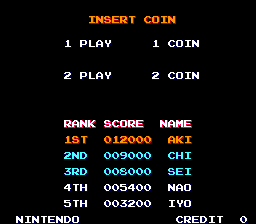
\includegraphics[width=0.25\textwidth]{img/highscore}};
\end{tikzpicture}
\end{Slide}








\end{document}







